\documentclass[12pt]{article}
\usepackage{natbib}
\usepackage{hyperref}
\usepackage{grffile}
\usepackage{graphicx}
\usepackage{subcaption}
\usepackage{amssymb,amsmath,amsthm}
\usepackage{xcolor}
\usepackage{xspace}
\usepackage[nameinlink,capitalize]{cleveref}
\usepackage{cleveref}
\usepackage[margin=1in]{geometry}
\usepackage{lineno}\renewcommand\thelinenumber{\color{gray}\arabic{linenumber}}
\usepackage{pdflscape}
\usepackage{enumerate}

% parameter values
\newcommand{\betaparam}{0.5}
\newcommand{\gammaparam}{0.2}
\newcommand{\invgammaparam}{6.0}
\newcommand{\Rnumparam}{3.0}
\newcommand{\rparam}{0.3}



% https://tex.stackexchange.com/questions/12703/how-to-create-fixed-width-table-columns-with-text-raggedright-centered-raggedlef
\usepackage{array}
\newcolumntype{L}[1]{>{\raggedright\let\newline\\\arraybackslash\hspace{0pt}}m{#1}}
\newcolumntype{C}[1]{>{\centering\let\newline\\\arraybackslash\hspace{0pt}}m{#1}}
\newcolumntype{R}[1]{>{\raggedleft\let\newline\\\arraybackslash\hspace{0pt}}m{#1}}

\usepackage{xspace}

\newcommand{\fref}[1]{Fig.~\ref{#1}}
\newcommand{\appref}[1]{Appendix~\ref{app:#1}}
\newcommand{\Rlogo}{R\xspace}
\newcommand{\percap}{\emph{per capita}\xspace}
\newcommand{\Rnum}{\ensuremath{\mathcal{R}_0}\xspace}
\newcommand{\covid}{COVID-19\xspace}
\newcommand{\pro}[1]{\ensuremath{\frac{\partial #1}{\partial \rho}}}
\newcommand\pder[2]{\ensuremath{\frac{\partial#1}{\partial#2}}} %\pder y{x}

\newcommand*\subtxt[1]{_{\textnormal{#1}}}
%% Roman subscript
\DeclareRobustCommand\_{\ifmmode\expandafter\subtxt\else\textunderscore\fi}

\newcommand{\comment}{\showcomment}
\newcommand{\showcomment}[3]{\textcolor{#1}{\textbf{[#2: }\textsl{#3}\textbf{]}}}
\newcommand{\nocomment}[3]{}

\newcommand{\fady}[1]{\comment{cyan}{Fady}{#1}}
\newcommand{\ali}[1]{\comment{magenta}{Ali}{#1}}
\newcommand{\jd}[1]{\comment{blue}{JD}{#1}}
\newcommand{\david}[1]{\comment{orange}{DJDE}{#1}}
\newcommand{\bmb}[1]{\comment{red}{BMB}{#1}}
\newcommand{\todo}[1]{\comment{red}{TODO}{#1}}

\theoremstyle{definition} % amsthm only
\newtheorem{proposition}{Proposition}
\newtheorem{theorem}{Theorem}

\bibliographystyle{apalike}

\title{Testing and Isolation Efficacy:\\Insights from a Simple Epidemic Model}
\author{\david{??? authors ??? affiliations ???}}

\begin{document}
\maketitle

\linenumbers

% %%%%%%%
\section{Abstract}

\bmb{abstract needs another editing pass, skipping for now}
\david{This needs substantial tightening.}

The effect of testing processes, including testing and test reporting, on epidemic dynamics, involving infection and recovery, can be studied at the individual level or the community level (e.g., nursing homes, long-term-care facilities, etc.).
Gaining insights to determine the sensitivity of the epidemic dynamics with respect to the testing processes will depend on underlying factors including the level of focus (individual or community), assumptions (model), and the interplay between these factors. 
In particular, fast testing and test reporting may be beneficial at the community-level, supported by many studies, as it gives a rapid assessment of the situation, identifies hot spots, and may enable rapid contact-tracing. However, the potential advantage of a slow rate of test return on the dynamics of an epidemic is real, often neglected, and needs to be quantified. At the individual level, this advantage can manifest in the following sense: individuals awaiting their test results or who have tested positive may partially or fully self-isolate, thus reducing or eliminating their transmission potential.
In this paper, we investigated this individual-level effect of testing processes on the epidemic dynamics by developing a SIR-type model.
Although the model development was motivated by the \covid epidemic, the model has general epidemiological and testing structures. The realistic components of the model include \percap testing intensity, test sensitivity and specificity, rate of test return, and isolation efficacy (i.e., reduction of the transmission probability by isolating individuals). The novel component is the compartment-specific relative testing weights, which reflect the testing strategies --- surveillance, diagnosis, or control. Here, we compare two testing strategies, random vs. targeted, and concluded that increasing testing “focus” from random to targeted always decreases \Rnum. Further, the following processes always decreases $\Rnum$; increasing the isolation efficacy parameters for tested and confirmed individuals, higher testing intensity if testing is random or testing intensity is small, and a higher rate of test return if the isolation efficacy for tested-awaiting individuals is low.

% %%%%%%%
\section{Introduction}

The observed dynamics of the \covid epidemic have been driven both by epidemiological processes (infection and recovery) and by testing processes (testing and test reporting). In addition to shaping epidemic observations (via case reports), testing processes also alter epidemiological dynamics. Because individuals with confirmed infections (positive tests) are likely to self-isolate, and individuals who are awaiting the results of a test may also do so, testing will generally increase the number of people who are isolating and hence reduce epidemic growth rates. We developed a mechanistic model that incorporates epidemic processes and testing in order to explore the effects of testing and isolation on epidemic dynamics.

If testing influences behavior, then epidemic dynamics will depend on who gets tested.
The impacts of testing will depend both on testing intensity (tests performed per day) and on how strongly testing is focused on people who are infectious.
This level of focus depends in turn on the purpose and design of testing programs. 
When testing is done for the purposes of disease surveillance \citep{foddai2020base}
tests are typically conducted randomly (or using a stratified random design) across the population in order to make an unbiased assessment of population prevalence.

Over the course of the \covid pandemic, however, the vast majority of testing has been done with other goals --
primarily diagnostic (determining infection status for clinical purposes), or for control (determining  infection status in order to isolate cases that have been found by contact tracing), which we characterize as \emph{targeted} testing strategies.
In these cases, testing probabilities can differ sharply across epidemiological compartments; in our dynamical model, we will characterize these probabilities by assigning a testing weight to each compartment that determines the \emph{relative} probability that an individual in that compartment will be selected for testing (see Methods). 

Diagnostic testing focuses on people with infection-like symptoms; thus the relative testing weights for infected people will depend on the relative probability of infected people having symptoms. For \covid infection, the testing weights will depend on the proportion of asymptomatic infections, the time spent pre-symptomatic vs.\ symptomatic during the course of an infection, and on the incidence of \covid-like symptoms among people in the population \emph{not} infected with \covid. Testing for epidemic control focuses on known contacts of infected people; in this case the testing weights for infected vs.\ uninfected people will depend on the probability of infection given contact, as well as the effectiveness of the system for identifying suspicious contacts.

When a new infectious disease emerges, it is important to determine whether it will grow exponentially in a susceptible population, and if so at what rate $r$.  The condition for positive exponential growth ($r>0$) is commonly expressed as $\Rnum>1$, where the basic reproduction number $\Rnum$ is the expected number of secondary infections arising from a typical infective individual in a completely susceptible population \citep{dietz1993estimation}.  Although the value of $\Rnum$ cannot completely characterize the dynamics of even the simplest epidemic model \citep{shaw2021what}, \david{well, technically it does up to rescaling time} it does give a simple and widely accepted index for the difficulty of control, as well as an indication of the likely final size of an epidemic \citep{ma2006generality}.

In order to understand the effect of testing processes on epidemic dynamics, we expanded one of the simplest mechanistic epidemic model---the standard deterministic SIR model---to include testing components. This model provides a sensible platform to link the modeling of epidemic and testing components and study their interaction. We studied the effects of testing intensity, rate of test return, and isolation efficacy, on transmission probability and epidemic dynamics when different levels of testing focus (from random to highly targeted) are in place.

% %%%%%%%
\section{Methods}

Our model groups individuals based on disease status (Susceptible, Infectious or Recovered) and testing status (\emph{untested}, waiting-for-\emph{positive}, waiting-for-\emph{negative}, or \emph{confirmed positive}) (\fref{fig:flowchart}).  The testing status of an individual in a given disease compartment $X$ (where $X \in \{S,I,R\}$) is denoted by a subscript, namely $X\_u$, $X\_p$, $X\_n$ and $X\_c$, for \emph{untested}, waiting-for-\emph{positive}, waiting-for-\emph{negative}, or \emph{confirmed positive}, respectively.  Two `accumulator' compartments, $N$ and $P$, are included in order to collect cumulative reported negative or positive tests. The model equations \eqref{model} and details of calculation of the basic reproduction number $\Rnum$ are presented in \appref{R0}.

\begin{figure}
\begin{center} 
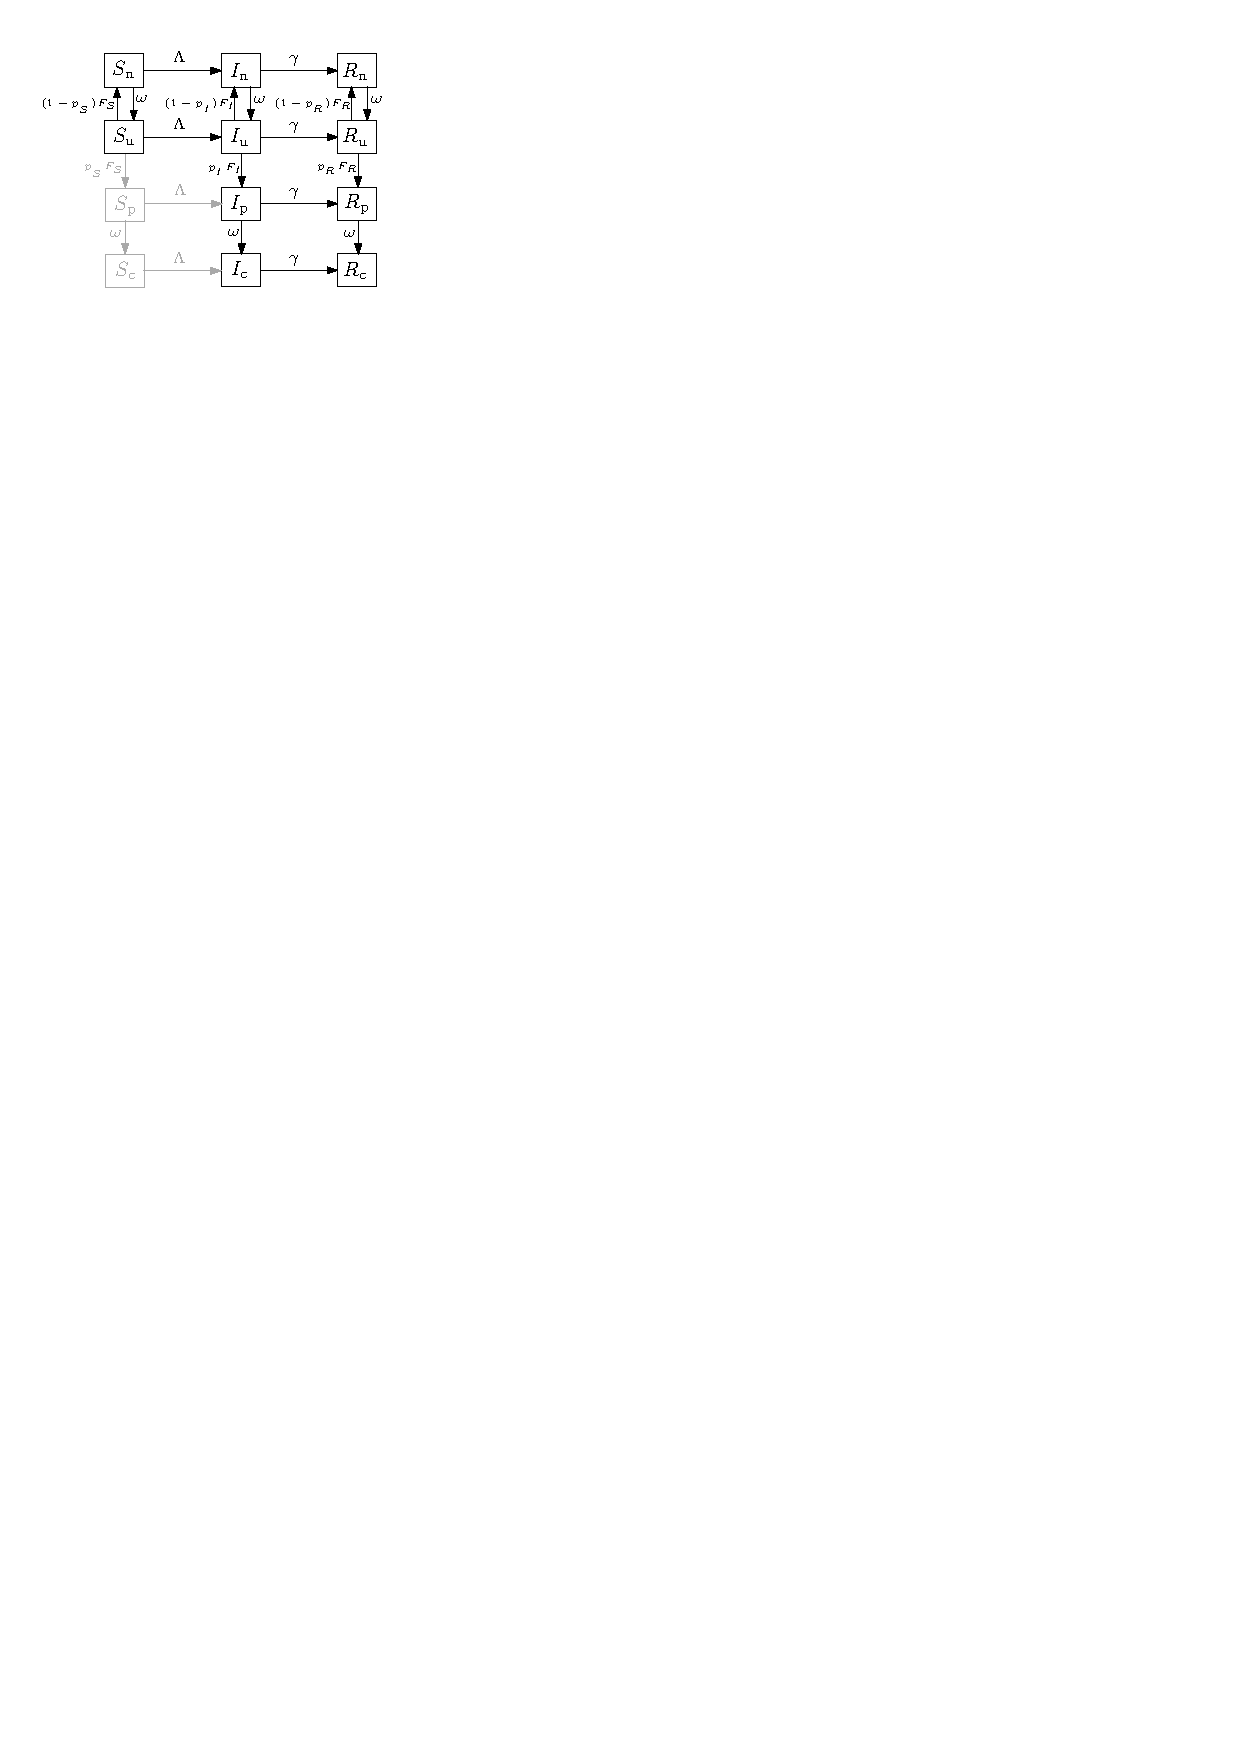
\includegraphics[scale=1.5]{pix/sir_comp.pdf}
\caption{\small Flowchart of the SIR (Susceptible-Infectious-Recovered) model, \ref{model}. The disease-based status of a compartment $X$ ($X \in \{S,I,R\}$) is combined with the testing status including $X\_u$, $X\_p$, $X\_n$ and $X\_c$, for \emph{untested}, waiting-for-\emph{positive}, waiting-for-\emph{negative}, or \emph{confirmed positive}, respectively. The force of infection is denoted by $\Lambda$ (Eq.~\eqref{Lambda}); $\gamma$ is the recovery rate; $\omega$ is the rate of test return; and $F_X$ (Eq. \eqref{F}) and $p_X$ represent the \percap testing rate and the sensitivity (probability of positive tests), respectively, for compartment $X$. For further description of the parameters see \cref{tab:params}.
Note that there is a slight mismatch in the top-to-bottom order of the testing-based compartments of each disease-based compartment $X$ between this flowchart and the model equations \eqref{model}; here we have switched  $X\_u$ and $X\_n$ for visual clarity.
\label{fig:flowchart}}
\end{center} 
\end{figure}

Table~\ref{tab:params} defines the model parameters, which are generally \percap flows between compartments, or modifiers to these flow rates. The novel component of the model lies in the compartment-specific relative testing weights $w_S$, $w_I$ and $w_R$; these give the relative rates at which people in the $S$, $I$, and $R$ compartments are tested, respectively. Thus, we can specify different levels of testing focus from random (all weights equal) to highly targeted (higher weights in more intensively tested compartments). For example, $w_I/w_S=3$ means that infected individuals are tested at three times the \percap rate of susceptible individuals. 

In order to allow parameterization of the model by the total (overall) \percap testing rate, we define the weighted size of the testing pool $W = w_S S\_u + w_I I\_u + w_R R\_u$, and calculate a scaling parameter for testing as:
\begin{equation}
\label{sigma}
\sigma = \frac{\rho N_0}{W},
\end{equation}
where $\rho$ is the \percap testing intensity for the population, defined as the number of daily tests administered in a population of size $N_0$.
\david{Why $N_0$ rather than just $N$?}
Thus, the \percap testing rate for compartment $X \in \{S,I,R\}$ is 
\begin{equation}
\label{F}
F_X=\sigma w_X.
\end{equation}
\david{$F$ isn't a natural symbol for ``testing rate''.  How about $\mathcal T_X$?}
For a highly sensitive test, infected people typically flow through to the ``confirmed positive'' ($I\_c$, $R\_c$) compartments and are thus not considered for further testing. Over the course of the epidemic, a sufficiently large fixed testing rate as specified in \eqref{sigma} can exhaust the pool of people available for testing, leading to a singularity when too few people are left untested to support the specified rate. Although this phenomenon does not affect our analysis of $\Rnum$, it can affect model dynamics (we present an adjustment to the model that solves this problem in \appref{singularity}).

The classical SIR model assumes a well-mixed population; homogeneity of the population (i.e., all individuals are equally susceptible and equally infectious with the same recovery rate when infected); exponentially distributed duration of infection; and large population size \citep{keeling2011modeling}. In addition to these standard assumptions, our model assumes: 
\begin{enumerate}[(i)]
\item there is a single force of infection (new \david{infections} per unit time \david{per susceptible}), $\Lambda$, defined as
  \begin{equation}
  \label{Lambda}
  \Lambda=\frac{\beta}{N_0} \big(I\_u + (1-\theta\_w)(I\_n+I\_p) + (1-\theta\_c)I\_c \big),
  \end{equation}
  with transmission rate $\beta$; $\theta\_w$ is the isolation efficacy (reduction of the probability of transmission) for individuals waiting for test results, while $\theta\_c$ is the isolation efficacy for individuals who have received a ``confirmed'' positive test (Table~\ref{tab:params}). Susceptible individuals who are waiting for test results experience an additional transmission reduction factor of $1-\theta\_w$ (\fref{fig:flowchart}). 
\item confirmed-positive individuals isolate at least as effectively as those awaiting test results, i.e.,
$$0\leq\theta\_w\leq\theta\_c\leq 1.$$ 
\end{enumerate}
For simplicity we assume that tests are perfectly \emph{specific} --- uninfected individuals never test positive ($p_s=0$). Thus there are no waiting-for-positive or confirmed-positive susceptible individuals, which reduces the number of model states from 12 to 10.

\begin{table}[htp]
\centering
\begin{tabular}{|c|L{2in}cc|} \hline
  Symbol & Description & Unit & Value \\ \hline
  $N_0$     & Total population size & people & $10^6$ \\ \hline
  $\omega$  & Rate of test return, i.e., rate of onward flow from ``waiting'' to ``confirmed'' or ``untested'' compartments  & 1/day & - \\ \hline
  $\gamma$ & Recovery rate & 1/day & 1/6 \\ \hline 
  $\rho$   & \percap testing intensity & 1/day & - \\ \hline 
  $\theta\_w$ & Isolation efficacy (reduction of the transmission probability) for ``waiting'' individuals & - & - \\ \hline
  $\theta\_c$ & Isolation efficacy for ``confirmed positive'' individuals & - & -  \\ \hline
  $\beta$ & Transmission rate & 1/day & 0.5 \\ \hline
  $\Lambda$ & Force of infection & 1/day & - \\ \hline
  $p_S$ & Probability of positive tests for $S$ ($= 1-\textrm{specificity}$) & - & 0 \\ \hline
  $p_I$ & Probability of positive tests for $I$ ($= \textrm{sensitivity}$) & - & 1 \\ \hline
  $p_R$ & Probability of positive tests for $R$ ($= 1-\textrm{specificity}$) & - & 0.5 \\ \hline
  $w_S, w_I, w_R$ & Relative testing weights & - &
  \begin{minipage}[t]{0.21\columnwidth}%
    Random: $\{1,1,1\}$ \\ Targeted: $\{0.3,1,1\}$
  \end{minipage} \\
  \hline
  \end{tabular}
\caption{\label{tab:params} Parameters of the model specified in \eqref{model}; see also \fref{fig:flowchart}.}
\end{table}

The Disease-Free Equilibrium (DFE) for the expanded SIR model (Eqs.~\ref{model}) is found by setting the infected compartments to 0 and solving for the unknowns. The DFE is
\begin{equation}
\label{dfe}
S\_n^*= \frac{\rho}{\omega} N_0, \ S\_u^*= N_0-S_n^*, \text{~and~} I_j=R_j=0 \ \text{for all }j.
\end{equation}
The corresponding \percap testing rate (Eq.~\ref{F}) for the infected compartment $I$ at DFE is one of the key analysis parameters and can be simplified as 
\begin{equation}
\label{eq:fi}
\hat F_I = (\omega\rho/(\omega-\rho))w_I/w_S \quad .
\end{equation}

The basic reproduction number, $\Rnum$, was calculated by using the next-generation matrix method \citep{van2002reproduction}. We present $\Rnum$ as
\begin{equation}
\label{R0}
\Rnum= \frac{\beta}{\gamma} \left(1-\Delta\right), 
\end{equation}
where the term $\beta/\gamma$ is the classical basic reproduction number for a simple SIR model \citep{keeling2011modeling}, and $0 < \Delta < 1$ is the proportional reduction \david{actually $1-\Delta$ is the proportional reduction; you should refer to this as the effectiveness of control, as you do below} due to testing and isolation processes, calculated as 
\begin{equation}
  \label{eq:del4a}
  \Delta= \frac{1}{C N_0}\big(C_1 S\_u^*+(C_2(1-\theta\_w)+C \theta\_w)S\_n^*\big),
\end{equation}
where
\begin{align}
\label{eq:C12}
C_{\phantom 1} &= (\omega+\gamma) \Big(\gamma(\omega+\gamma)+(\gamma+\omega p_I)\hat F_I\Big),\\
C_1 &= (\omega+\gamma)(\theta\_w \gamma+\theta\_c \omega p_I) \hat F_I,\\
C_2 &= \Big( \omega\gamma(1+p_I)\hat F_I+\gamma^2(\omega+\gamma+\hat F_I)\Big)\theta\_w + \omega^2p_I\hat F_I\theta\_c.
\end{align}
(\appref{R0} gives a detailed derivation of these expressions.)
This explicit formula enables us to study the effects of testing and isolation parameters on $\Rnum$ both analytically and via numerical solutions.
We are specifically interested in parameters that could be manipulated by public health policy: isolation efficacy, $\theta\_c$ and $\theta\_w$; \percap testing intensity, $\rho$; and the rate of test return, $\omega$. In particular, we look at the partial derivatives of $\Delta$ with respect to these parameters (\appref{rho}). 
We derived general expressions for these derivatives. However, we analyzed the effect of $\omega$ on $\Delta$ for the special case of low testing intensity. Specifically, by making the restriction $\rho \ll 1$, we are able to Taylor-expand $\Delta$ at $\rho=0$, use the linear approximation with respect to $\rho$ and analyze the resulting simplified derivatives to illustrate a surprising non-monotonic relationship between $\Delta$ and $\omega$. 

Analytic calculation of the next-generation matrix and simplification of the $\Rnum$ expression, were performed in Maple\textsuperscript{\texttrademark} \citep{maple14}; numerical calculation and contour plots were done in R \citep{r}.
We computed the values and contours of $\Delta$ at both low (\fref{pan}) and high (\fref{pan2}) testing intensities, and for both random testing ($w_S=w_I=w_R=1$) and targeted testing ($w_S=0.3$; $w_I=w_R=1$).

\jd{Why do we use a different range of $\omega$ for the two cases?}\ali{added a sentence to the end of this paragraph to address this (I hope).}
The low-testing case \fref{pan} reflects the case where testing intensity $\rho$ is small relative to the population size. Specifically, $\rho \in [0,0.013]$, and test return rate $\omega\in [1/12,2]$. This testing intensity reflects realistic testing rates during the \covid pandemic, i.e., a maximum of 1.3\% of the population per day \david{If it is 4x larger than Ontario, what makes it ``realistic''?} (this is approximately four times the maximum testing rate in Ontario, Canada in mid-2021). The less realistic high-testing case \fref{pan2} is included to highlight the occurrence of non-monotonic changes in $\Rnum$ with respect to $\rho$.
In \fref{pan2} the maximum capacity of $\rho$ is larger relative to the population size, $\rho \in [0,1/5)$ and the test return rate $\omega\in [1/5,2]$; these values are clearly unrealistic for a large population but might be relevant for small populations undergoing focused testing, such as a sports league or university. In these figures, the implied baseline reproduction number (for the SIR model without testing) is $\Rnum=\frac{\beta}{\gamma}=3$. Note that the different range of test return rate $\omega$ for the two cases of low and high testing intensities is due to the restriction $\rho<\omega$ which is a requirement for feasible DFE (\ref{dfe}).
  
% %%%%%%%
\section{Results}

\jd{Should we talk less about \Rnum\ and keep the focus on $\Delta$? The back and forth is a bit tiring.}

We can use the formula for $\Rnum$ \eqref{R0} to make a number of straightforward inferences about parameters that affect $\Rnum$ monotonically, i.e., for which the associated partial derivative of $\Delta$ always has the same sign (see Appendices).

\begin{enumerate}

\item \label{p1:eta} Increasing isolation efficacy for waiting ($\theta\_w$) and confirmed-positive ($\theta\_c$) individuals always decreases \Rnum (Eqs.~\ref{eq:del4_theta},~\ref{eq:d_del4_thetac},~\ref{eq:d_del4_thetaw});
\item \label{p1:rho} Higher testing intensity $\rho$ decreases $\Rnum$ if
%% \begin{enumerate} \item
testing is random (all $w_X$ equal) or testing intensity ($\rho$) is small (Eq.~\ref{eq:dd3dr}).
%% \end{enumerate}
\item \label{p1:omega} Increasing the rate of test return ($\omega$) always decreases \Rnum if waiting individuals do not isolate ($\theta\_w=0$) (Eq.~\ref{eq:dlindo}).
\item \label{p1:w} Increasing testing focus, i.e., changing the testing weights from random ($w_S=w_I$) toward targeted  ($w_S<w_I$), always decreases \Rnum (Eq.~\ref{eq:d_del_wis}).
\end{enumerate}

\newpage
\begin{figure}[h!]
\centering
\begin{subfigure}[t]{.49\textwidth}
\centering
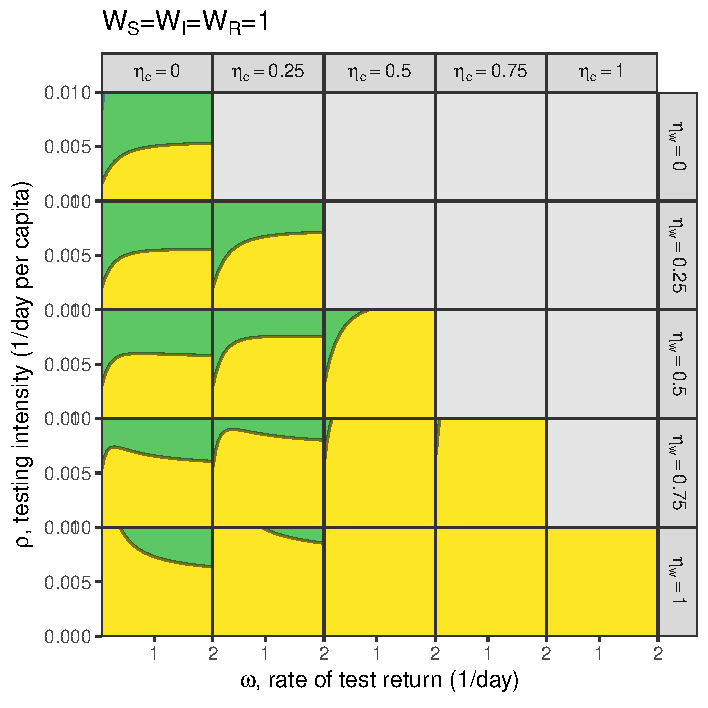
\includegraphics[width=\linewidth]{codes/R0contour_random.pdf}
\caption{}\label{p.a}
\end{subfigure}
%
\begin{subfigure}[t]{.49\textwidth}
\centering
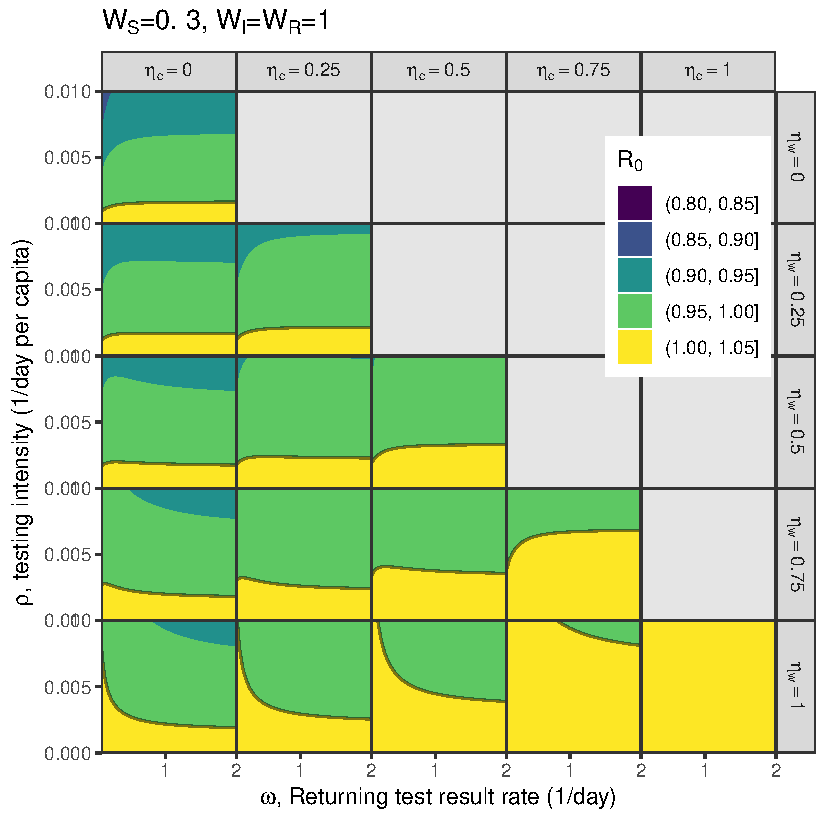
\includegraphics[width=\linewidth]{codes/R0contour_TTI.pdf}
\caption{}\label{p.b}
\end{subfigure}
\caption{
{\bf Effectiveness of testing and isolation in reducing $\Rnum$ at low \percap testing intensity ($\rho$).}
Numerical evaluation of the effectiveness of control ($\Delta$: eq.~\ref{eq:del4}\david{wrong eq ref}), over a range of testing and isolation parameters. Parameter values (Table~\ref{tab:params}):
$\beta=\betaparam/$day, $1/\gamma= \invgammaparam$ days (baseline $\Rnum=\Rnumparam$, $r=\rparam$); $\omega \in [1/12,2]/$day;  $\rho \in [0,0.013]/$day per capita; $\theta\_w$ and $\theta\_c$ vary between 0 (no effect of isolation) and 1 (complete elimination of transmission); $p_S=0$, $p_I=1$ and $p_R=0.5$. Only parameter sets where $\theta\_c \geq \theta\_w$ (confirmed-positive individuals isolate more effectively than waiting individuals) are shown; the alternative case, $\theta\_w > \theta\_c$, is unrealistic. Contours of $\Delta$ are plotted for (a) random testing ($w_S=w_I=w_R=1$) and (b) targeted testing ($w_S=0.3$; $w_I=w_R=1$). 
}
\label{pan}
\end{figure}

\begin{figure}[h!]
\centering
\begin{subfigure}[t]{.49\textwidth}
\centering
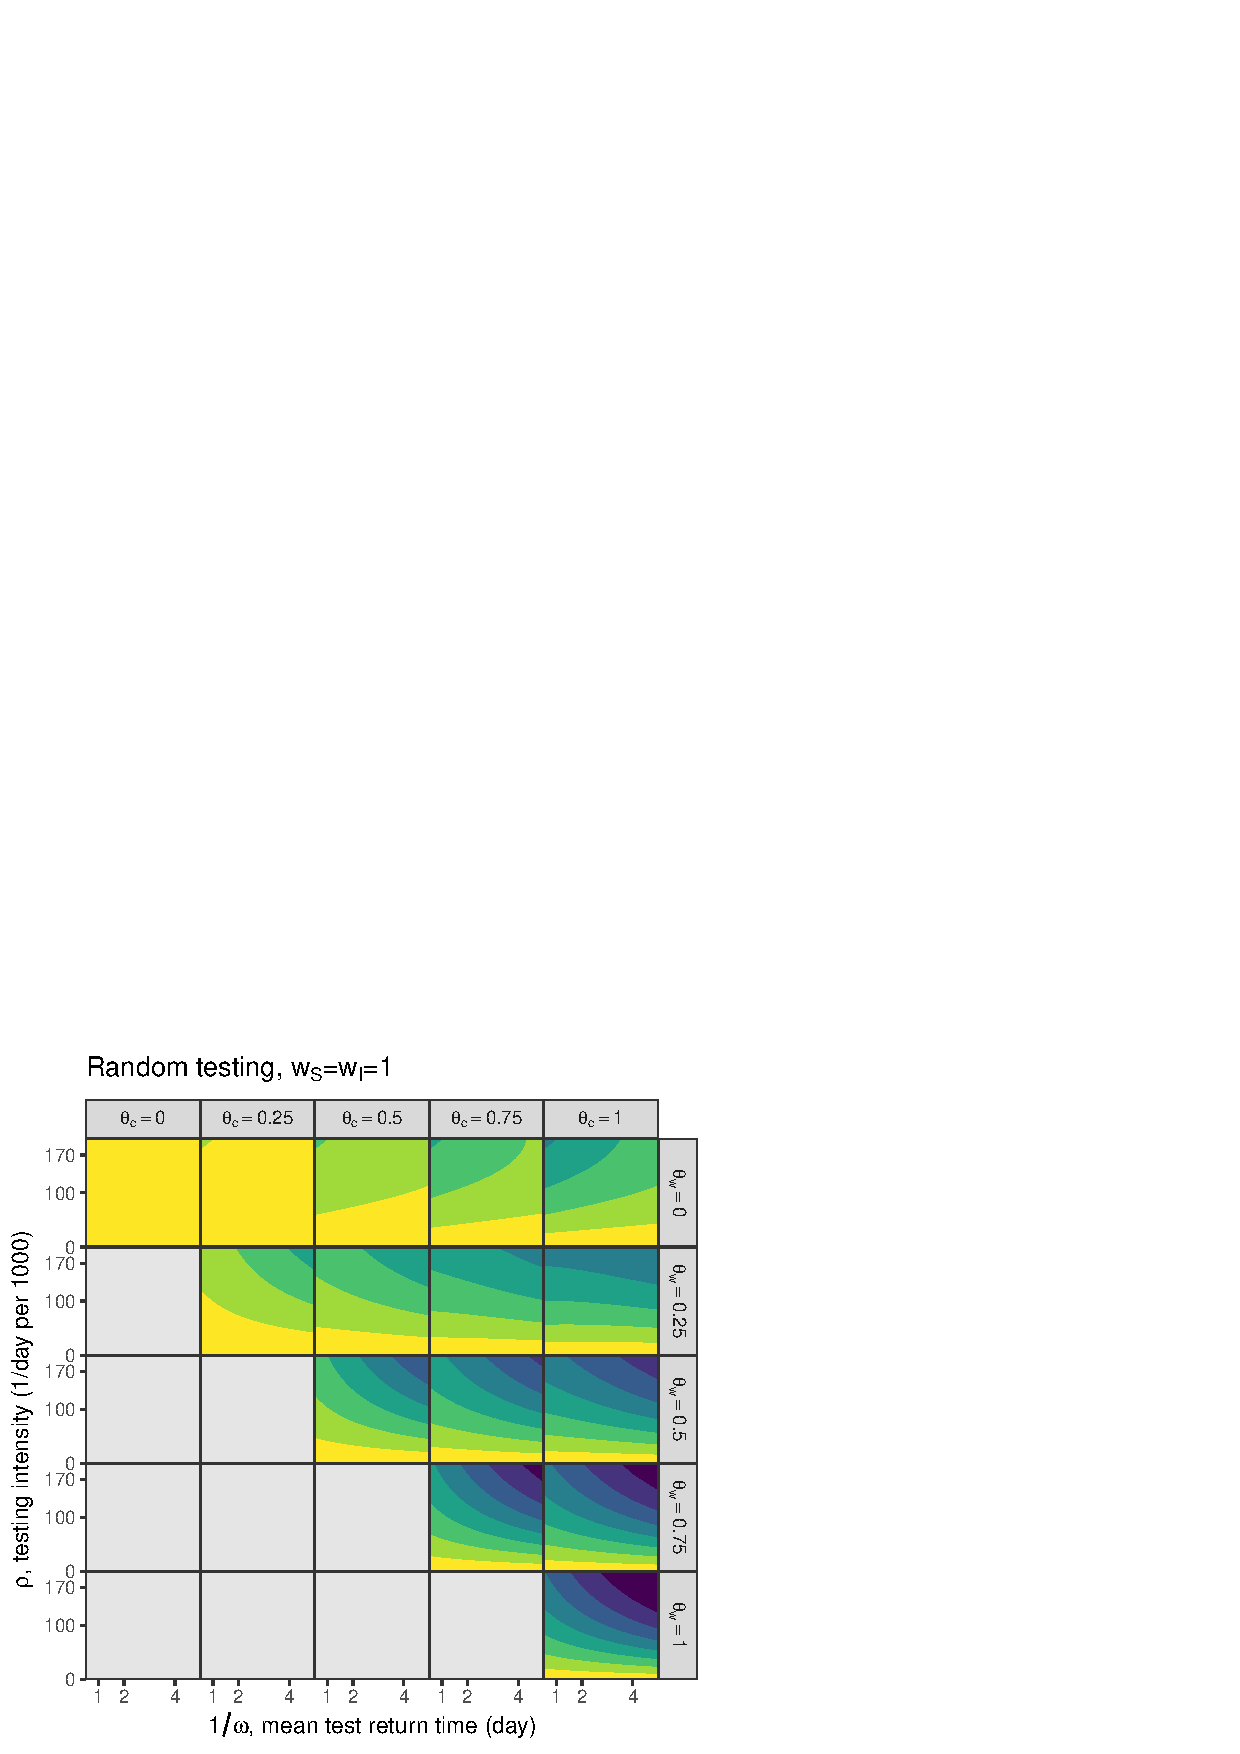
\includegraphics[width=\linewidth]{codes/R0contour_random2.pdf}
\caption{}
\end{subfigure}
%
\begin{subfigure}[t]{.49\textwidth}
\centering
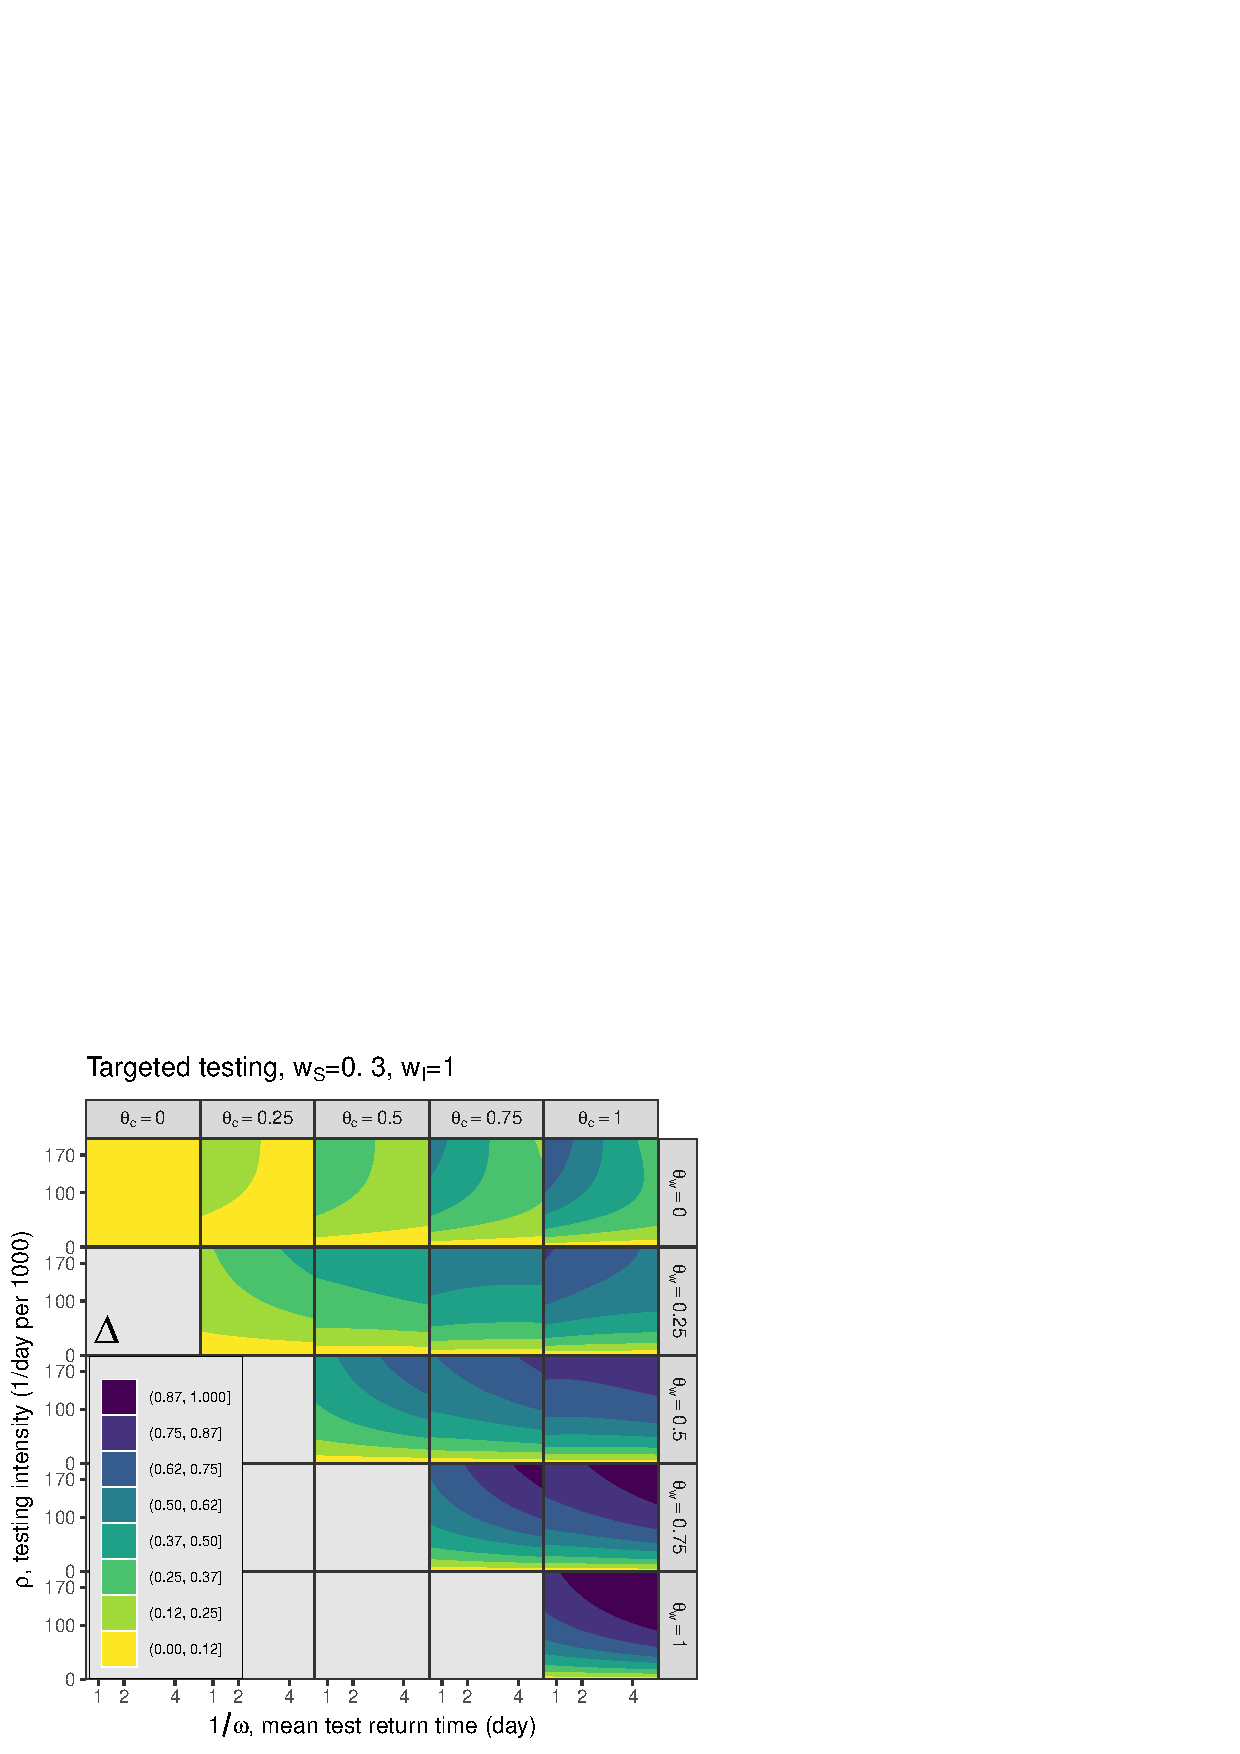
\includegraphics[width=\linewidth]{codes/R0contour_TTI2.pdf}
\caption{}
\end{subfigure}
\caption{
  {\bf Effectiveness of testing and isolation in reducing $\Rnum$ at high \percap testing intensity.}
  Numerical evaluation of the effectiveness of control ($\Delta$: eq.~\ref{eq:del4}\david{again wrong eq ref}), over a range of testing and isolation parameters. Parameters as in \fref{pan} except: $\omega \in [1/5,2]/$day, $\rho \in [0,1/5)/$day. As in \fref{pan}, subplots show (a) random testing where $w_S=w_I=w_R=1$ and (b) targeted testing where $w_S=0.3$ and $w_I=w_R=1$.
}
\label{pan2}
\end{figure}

However, there are also two specific cases where $\Delta$ changes non-monotonically, in counterintuitive directions, as a function of testing and isolation parameters.

\begin{itemize}
\item We would generally expect increasing testing delays to increase \Rnum, thus decreasing effectiveness of control $\Delta$. This is in fact what happens when waiting individuals do not isolate ($\theta\_w =0$, top row of \fref{pan}) --- as we move to the right within each plot in this row, $\Delta$ decreases.
However, when waiting individuals isolate ($\theta\_w>0$), we more often see the opposite effect: longer testing delays lead to a greater control effect $\Delta$ (reduced $\Rnum$). The reason is that people waiting for negative tests are assumed to continue to isolate; this applies both to susceptibles and to people who became infected while waiting for negative test results. This effect outweighs the effect of confirmed individuals isolating, except when this isolation parameter ($\theta\_c$) is substantially greater than $\theta\_w$. This result depends on the idea that, all else equal, people who have to wait longer for test results isolate at the same level (but for a longer time) as they would if the wait were shorter.
\item \fref{pan} also shows that greater testing intensity (increasing $\rho$) generally increases the effectiveness of control (moving up in each panel). However, this relationship can be reversed at very high testing intensities (provided testing is targeted, and $\theta\_w$ is relatively small; \fref{pan2}(b), right three panels of top row). It is theoretically possible for increasing testing intensity to \emph{increase} \Rnum because more rapid testing leaves more susceptibles in the ``waiting-for-negative-results'' category at the DFE; if these people become infected while waiting, they will need to wait for their negative test result before they can be tested again, receive a positive test, and then begin self-isolating. This effect is usually weak compared to the beneficial effects of testing.

\end{itemize}
  

%%%%%%%%%%%%
\section{Discussion}

In this paper, we have defined and analyzed a simple compartmental model that combines epidemiological dynamics (as defined by a simple SIR model) with the dynamics of testing and isolation. Our model is a caricature --- it models the most basic feedbacks between epidemic and testing processes, but does not attempt to incorporate the many known complications of COVID-19 epidemiology (e.g. exposed, presymptomatic, and asymptomatic compartments \citep{kain2021chopping}; time-varying testing rates [REFS?]; behavioural dynamics \citep{weitz2020awareness}). Thus, it is most appropriate for assessing the \emph{qualitative} phenomena that arise from the interactions between epidemiology and testing, rather than for making quantitative predictions or guiding pandemic responses.

Many of the qualitative results we have derived confirm simple, common-sense intuitions. In particular, we can generally decrease $\Rnum$ by increasing isolation efficacy or testing intensity; returning tests faster, if individuals do not isolate while they are waiting for results; or increasing testing focus to target individuals who are likely to be infectious (e.g. symptomatic people or close contacts of known infections).

However, we did find two surprising patterns: longer delays in returning tests can decrease the spread of the epidemic, and increasing testing rates can increase its spread.

Over a broad range of parameter space (for random testing, approximately $\theta\_w \geq 0.25$; for targeted testing, $\theta\_w \geq 0.25$ and either $\theta\_c \ge 0.5$ or $1/\omega > 5$), decreasing $\omega$ --- i.e., decreasing the rate at which tested people find out about their infection status --- decreases $\Rnum$. This result is counterintuitive; public health agencies have invested a lot of effort in increasing this rate. Dynamically, this effect occurs because speeding up test returns shortens the isolation period of uninfected individuals. For infected people it only shortens the time to progression to the isolation level of the confirmed-positive compartment. Slowing test returns increases $\Rnum$ only if the proportion of infectives in the tested population (test positivity), and the magnitude of increase in isolation effectiveness from the waiting to the confirmed-positive compartment, are large enough to outweigh the decrease in isolation of uninfected waiting individuals.

While slowing test returns does decrease $\Rnum$ over a broad range of parameter space in our model, there are several real-world processes missing from our model that make it implausible that slowing test returns would actually be an effective public health measure. First, our model is missing the components that would allow us to model the primary benefit of rapid testing, i.e. detecting and containing outbreaks while they are still in progress. This process could be modeled phenomenologically by making the testing focus increase as an increasing proportion of cases are detected, because finding infections allows tests to be concentrated on their connections. Second, in the real world individuals become less likely to maintain isolation if they are required to do so for longer; phenomenologically, we could allow  effectiveness of isolation while waiting for test returns to be an increasing function of test return speed, or we could introduce a separate ``waiting, but no longer isolating'' compartment that individuals entered from the ``waiting, isolated'' compartment at a specified rate. Third and finally, if one wants to decrease the overall transmission rate of the population there are more effective methods than keeping tested people in limbo -- these include masking, ventilation, distancing measures, retail and event closures, or stay-at-home orders.

The other counterintuitive result from our analysis is that, for sufficiently high testing intensity $\rho$, increasing testing intensity can actually increase $\Rnum$ (e.g. \fref{pan2}(b), upper right panel [$\theta\_c=1$, $\theta\_w=0$]). This phenomenon occurs mainly because of a peculiar feature of the DFE in our model: we assume that testing is ongoing before the beginning of the epidemic, so that the starting point of the epidemic invasion is an equilibrium distribution of susceptibles between the $S\_n$ (untested) and $S\_u$ (waiting) compartments: in particular, $S\_u^* = \rho/(\rho + \omega)$. (In reality, testing intensity itself is a dynamic variable that will increase as the epidemic proceeds.) If isolation in the waiting compartment is low ($\theta\_w \ll 1$), then waiting individuals can easily be infected once the epidemic starts. Once infected they can still infect others while in the waiting compartment, and cannot be tested again before they have returned to the untested compartment. Thus, under certain extreme conditions (low $\theta\_w$, high $\theta\_c$, low $\omega$, high $\rho$), $\Rnum$ becomes an increasing function of testing intensity. \bmb{This phenomenon occurs primarily (only??) for targeted testing, because \ldots CAN WE FIGURE OUT WHY? Targeting should be irrelevant to determining the DFE (because everyone is $S$ at that point), so what is the dynamical explanation? Is there a second order effect somewhere, e.g. testing is more effective overall (darker colours in Fig 3(b) upper-right panel than in Fig 3(a) upper panel), so we more quickly reach the point where the effect of increasing $S\_n^*$ outweighs the beneficial effects of testing?} However, this phenomenon is even more unrealistic than the possibility that slowing test returns increases $\Rnum$. It depends both on the assumption that regular testing is occurring before the epidemic starts, and on levels of testing that are unrealistically high (at least in large, general-population settings), i.e. at least 10\% of the population being tested per day.

Although we model the testing process in more detail than most mathematically focused epidemiological models, one place where more detail could be informative is in the processes determining the testing weights $\{w_S, w_I, w_R\}$. While random testing, as done for surveillance purposes, unambiguously leads to equal testing weights, making precise quantitative connections between public health practices and testing weights is difficult in other contexts. The testing weights reflect the correlation between an individual's risk of infection and their likelihood of being tested due to age, occupation, geographic location, etc.. This correlation is influenced, among many other factors, by the proportion of the uninfected population with COVID-like symptoms (e.g. due to seasonal upper respiratory tract infections); the concentration of transmission and testing in hot spots such as long-term care facilities and high-density workplaces; the overall testing intensity (and hence e.g. restriction to symptomatic individuals); and the proportion of COVID-infected people who are symptomatic. Future steps should explore mathematically tractable ways to model some of these factors more precisely. For example, separating the infected class into exposed, symptomatic, and a- or pre-symptomatic compartments and allowing the testing weights to vary across non-symptomatic (exposed/asymptomatic/presymptomatic) vs. symptomatic compartments could reflect the allocation of tests to diagnostic purposes (targeting symptomatic individuals) vs. contact-tracing (targeting infected but non-symptomatic individuals) vs. screening (relatively equal weights, depending on the venue). Alternatively, one could make the testing weights depend on the testing intensity or test return rate as suggested above. Whatever complexity is added would probably put the model beyond reach of the analytical methods we have used in this paper, but one could still use semi-numerical methods such as constructing the next-generation matrix and using it to evaluate the derivatives of $\Rnum$ with respect to the parameters numerically.

Although testing and tracing is a key part of infection control strategy, mathematical epidemiologists have typically analyzed it with detailed models designed to inform particular public health efforts, rather than analyzing simple but general models of the feedback between testing and epidemic dynamics \bmb{can we back this statement up? more general citations to test-and-trace? HIV? Bergstrom et al might be a counterexample, although it's for a different context [repeated testing of an isolated population]}. \ali{the following sentences added to address Ben' comment:} There have been several modeling works of testing and tracing dynamics and their interaction with epidemiological dynamics. In the context of repeated screaning and random testing of isolated populations (such as a university setup), \cite{bergstrom2020frequency} provided some analytical results, \cite{rogers2021high} simulated a SEIR model with high-low testing intensity and sensitivity. Further, \cite{friston2021testing} model the effects of self-isolation on testing and tracking. Our modeling approache is novel compared to these works. We hope that this paper will inspire further explorations of the fundamental properties of dynamical systems that incorporate explicit testing models in an epidemiological context. \bmb{we could also talk about test and trace as a 'speed' intervention, but I'm tired}.

\bmb{Leftover comments:
\begin{itemize}
\item should emphasize (at some appropriate point in text) that $\Delta$ is independent of $\beta$ (and hence of $\Rnum$ if we are thinking primarily of holding $\gamma$ constant and varying $\beta$) for the small-$\rho$ (Taylor-expansion) case, see Eq.~\ref{eq:lin}.
\item it would be good to have a few more testing refs: Bergstrom et al., there might be some other stuff we can recycle from the lab meeting review; Friston's stuff deserves to be mentioned because it does have explicit testing flows too. We should try not to ignore/piss anyone off who has already done stuff
\end{itemize}
}
\ali{In respense to Ben's comment}





% %%%%%%%
\bibliography{SIRlibrary}

% %%%%%%%%%%%%%%%%%%%%%%%%%%%%%%%%%%%%%%%%%%%%%%%%%%%%%%%%%%%%%%%%%%
\clearpage
% \widetext
\appendix
\section{Appendix}
\setcounter{equation}{0}
\setcounter{figure}{0}
\setcounter{table}{0}
% \setcounter{page}{1}
\makeatletter
\renewcommand{\theequation}{A\arabic{equation}}
\renewcommand{\thefigure}{A\arabic{figure}}
\renewcommand{\bibnumfmt}[1]{[A#1]}
\renewcommand{\citenumfont}[1]{A#1}

\subsection{Model and calculation of $\Rnum$}\label{app:R0}

The model in the form of a system of ordinary differential equations is 
\begin{subequations}\label{model}
\begin{align}
 d S\_u/dt &= -\Lambda S\_u - F_S S\_u + \omega S\_n, \\
 d S\_n/dt &= -(1-\theta\_w)\Lambda S\_n + (1-p_S) F_S S\_u - \omega S\_n, \\
 d S\_p/dt &= -(1-\theta\_w)\Lambda S\_p + p_S F_S S\_u - \omega S\_p, \\
 d S\_c/dt &= -(1-\theta\_c)\Lambda S\_c + \omega S\_p, \\
 d I\_u/dt &= \Lambda S\_u - F_I I\_u + \omega I\_n  - \gamma I\_u, \\
 d I\_n/dt &= (1-\theta\_w)\Lambda S\_n + (1-p_I) F_I I\_u - \omega I\_n -\gamma I\_n, \\
 d I\_p/dt &= (1-\theta\_w)\Lambda S\_p + p_I F_I I\_u - \omega I\_p -\gamma I\_p, \\
 d I\_c/dt &= (1-\theta\_c)\Lambda S\_c + \omega I\_p - \gamma I\_c, \\
 d R\_u/dt &= \gamma I\_u - F_R R\_u + \omega R\_n, \\
 d R\_n/dt &= \gamma I\_n + (1-p_R) F_R R\_u - \omega R\_n, \\
 d R\_p/dt &= \gamma I\_p + p_R F_R R\_u  - \omega R\_p, \\
 d R\_c/dt&= \gamma I\_c + \omega R\_p, \\
 dN/dt &= \omega (S\_n + I\_n + R\_n),  \\
 dP/dt &= \omega(I\_p + R\_p) ,
\end{align}
\end{subequations}
%
(see Table \ref{tab:params} for parameter definitions). The next generation matrix for this model is $G = F V^{-1}$, where matrix $F$ represents the inflow of new infection to the infected compartments and matrix $V$ represents the flow in the infected compartments when the population is totally susceptible. 
Matrices $F$ and $V$ are
\begin{align}
\label{FV}
F =& \beta/N_0 \left[ \begin {array}{cccc} 
S\_u^* & (1-\theta\_w) S\_u^* & (1-\theta\_w) S\_u^* & (1-\theta\_c) S\_u^*\\
(1-\theta\_w)S\_n^* & (1-\theta\_w)^2 S\_n^* & (1-\theta\_w)^2 S\_n^* & (1-\theta\_w)(1-\theta\_c) S\_n^* \\ 
0&0&0&0\\
0&0&0&0
 \end {array} \right] \\
 =&\beta/N_0 \left[ \begin {array}{c} S\_u^* \\ (1-\theta\_w)S\_n^* \\ 0 \\ 0 \end {array} \right]
        \left[ \begin {array}{cccc} 1,   1-\theta\_w,   1-\theta\_w,   1-\theta\_c \end {array} \right], \text{and}\\  V=&
 \left[ \begin {array}{cccc}  
\hat F_I+\gamma&-\omega&0&0\\
-(1-p_I)\hat F_I&\omega+\gamma&0&0\\
-p_I \hat F_I&0&\omega+\gamma&0\\
0&0&-\omega&\gamma
\end {array} \right].
\end{align}
The matrix inverse of $V$ is 
\begin{align}
\label{vinv}
V^{-1} =&
\frac{1}{\gamma C}
\left[ \begin {array}{cccc}
\gamma(\omega+\gamma)^2 & \gamma\omega(\omega+\gamma)&0&0\\ \noalign{\medskip}
\gamma(\omega+\gamma)(1-p_I) \hat F_I & \gamma(\omega+\gamma)(\hat F_I+\gamma)&0&0 \\ \noalign{\medskip}
\gamma(\omega+\gamma) p_I \hat F_I & \gamma\omega p_I \hat F_I & C \gamma/(\omega+\gamma) & 0 \\ \noalign{\medskip}
\omega(\omega+\gamma) p_I \hat F_I & \omega^2 p_I \hat F_I & C \omega/(\omega+\gamma) & C
\end {array} \right],
\end{align}
where $C= \big( \gamma(\omega+\gamma)+(\gamma+\omega p_I)\hat F_I \big) (\omega+\gamma)$ and $\hat F_I$ is the \percap testing rate for the infected people and represented in Eq.~\eqref{eq:fi}. Note that all the columns of matrix $V^{-1}$ summ up to $1/\gamma$.

The particular form of $F$ with two rows of zeros at the bottom results in the following blocked form of matrix $G$.
\begin{equation}
\label{mat:G}
G = \left[ \begin {array}{cc}
G_{11}&G_{12}\\
0&0
\end {array} \right],
\end{equation}
where both blocked matrices $G_{11}$ and $G_{12}$ are 2 by 2. Given the upper triangular form of matrix $G$, the basic reproduction number $\Rnum$ (defined as the spectral radius of matrix $G$) is only determined by the blocked matrix $G_{11}$,
\begin{equation}
\label{G11}
G_{11} = \frac{\beta}{\gamma   C} 
\left[ \begin {array}{c} (\omega-\rho)/\omega \\ (1-\theta\_w)\rho/\omega \end {array} \right]
\left[ \begin {array}{cccc} 1,   1-\theta\_w,   1-\theta\_w,   1-\theta\_c \end {array} \right]
\left[ \begin {array}{cc}
\gamma(\omega+\gamma)^2 & \gamma\omega(\omega+\gamma)\\ \noalign{\medskip}
\gamma(\omega+\gamma)(1-p_I)\hat F_I & \gamma(\omega+\gamma)(\hat F_I+\gamma) \\ \noalign{\medskip}
\gamma(\omega+\gamma) p_I \hat F_I & \gamma\omega p_I \hat F_I \\ \noalign{\medskip}
\omega(\omega+\gamma) p_I \hat F_I & \omega^2 p_I \hat F_I
\end {array} \right].
\end{equation}
It is notable that matrix $F$ \eqref{FV} has rank one and consequently $G_{11}$ does so. That is $G_{11}$ has only one non-zero eigenvalue which is $\Rnum$.

The expression of $\Rnum$ has a complicated form with all of the model parameters involved. This expression can be simplified and represented given the specific form of matrix $G_{11}$ \eqref{G11}. For the purpose of simplicity we present $\Rnum$ in the manuscript in terms of expressions $C$, $C_1$ and $C_2$, specified in \eqref{eq:C12}. 

It remains hard to show that the reproduction number $\Rnum$ is decreasing with respect to \percap testing intensity, $\rho$, and the speed of the test return, $\omega$, for the feasible ranges of the parameters, that is
\begin{align}
\label{cond}
& \omega>0, \\
& 0 \leq \rho<\omega,\\ 
& 0 \leq \theta\_w \leq \theta\_c \leq 1, \\
& \frac{w_I}{w_S}\geq 1.
\end{align}
In realistic cases the testing rate $\rho$ is very small (i.e., only a small fraction of the population can be tested every day); it is thus reasonable to use a linear approximation of $\Rnum$ for $\rho \ll 1$ to analyze the behaviour of $\Rnum$ with respect to $\omega$ (see section \appref{omega}). 
In the next section we provide an equivalent representation of $\Rnum$ in order to show that increasing testing intensity typically decreases $\Rnum$.

% %%%%%%%
\subsection{More testing intensity may decrease $\Rnum$}\label{app:rho}

This section shows that $\pro{\Delta}$ can be positive or negative, with $\Delta$ defined in Eq.~\eqref{eq:C12}, and thus $\pro{\Rnum} < 0$, where $\Rnum$ is given in Eq.~\eqref{R0}. We rewrite matrix $G_{11}$ in \eqref{G11} in the following form to simplify the calculations:
\begin{equation}
\label{G112}
G_{11} = \frac{\beta}{\gamma C} 
\left[ \begin {array}{c}  S\_u^*/N_0 \\ (1-\theta\_w) S\_n^*/N_0  \end {array} \right]
\left[ \begin {array}{cccc} 
C-C_1, C-C_2\end {array} \right],
\end{equation}
where $C$ is the same as the one in Eq. \eqref{eq:C12}, i.e., 
$$C=(\omega+\gamma)(\gamma(\omega+\gamma)+(\omega p_I+\gamma) \hat F_I),$$
and $C_1$ and $C_2$ are 
\begin{align*}
% \label{eq:C12}
C_1 =& (\omega+\gamma)(\theta\_w   \gamma+\theta\_c  \omega  p_I) \hat F_I,\\
C_2 =& \big( \omega\gamma(1+p_I)\hat F_I+\gamma^2 (\omega+\gamma+\hat F_I)\big)\theta\_w + \omega^2 p_I \hat F_I \theta\_c,
\end{align*}
where $\hat F_I$ is given in Eq.~\eqref{eq:fi}.
Note that for analysis brevity, we let $N_0=1$, thus $S\_u^*$ and $S\_n^*$ are in the scale of 0 to 1.
$\Rnum$ is in the same form as in Eq. \eqref{R0}  
$$\Rnum= \frac{\beta}{\gamma} (1-\Delta),$$
where 
\begin{equation*}
\label{eq:del4}
\Delta= \frac{1}{C}\big(C_1 S\_u^*+(C_2(1-\theta\_w)+C \theta\_w) S\_n^*\big).
\end{equation*}

{\bf The first goal}
is to explore how changes in isolation, $\theta\_w$ and $\theta\_c$, affects $\Rnum$. Mathematically we would like to verify the sign of $\pder \Rnum{\theta\_w}$ and $\pder \Rnum{\theta\_c}$. We start with simplifying $\Delta$ \eqref{eq:del4} by factoring $\theta\_w$ and $\theta\_c$ in Eq.~\eqref{eq:del4}. Thus, $\Delta$ can be rewritten as
\begin{equation}
\label{eq:del4_theta}
\Delta= \frac{1}{C}\Big(
-D_1 S\_n^* \boldsymbol {\theta\_w^2}+
\big(-\omega^2 p_I \hat F_I S\_n^*\theta\_c+ D_2 S\_n^*+\gamma \hat F_I(\omega+\gamma) \big)\theta\_w+
(\omega+\gamma S\_u^*)\omega p_I \hat F_I \theta\_c
\Big),
\end{equation}
where
\begin{align}
\label{eq:del4_d1d2}
D_1=& (\omega+\gamma)\gamma^2+(\omega+\gamma+\omega p_I)\gamma \hat F_I, \\
D_2=& (3\omega+2\gamma)\gamma^2+(\omega+\gamma+2\omega p_I)\gamma \hat F_I+(\gamma+p_I \hat F_I)\omega^2.
\end{align}
$\Delta$, Eq.~\eqref{eq:del4_theta}, is linear in $\theta\_c$ with a positive coefficient. thus
\begin{equation}
\label{eq:d_del4_thetac}
\pder\Delta{\theta\_c}=1/C(\gamma S\_u^*+\omega(1-\theta\_w S\_n^*))\omega p_I \hat F_I.
\end{equation}
This results in increasing $\Delta$, thus decreasing $\Rnum$ with respect to $\theta\_c$, that is $\pder \Rnum{\theta\_c}\leq 0$. Note that $C$ is independent of $\theta\_c$ and $\theta\_w$. 

With a similar logic, $\Delta$ \eqref{eq:del4_theta} is a concave-down quadratic equation in $\theta\_w$, given by
\begin{equation}
\label{eq:del4_thetaw}
1/C \Big( -D_1 S\_n^*\theta\_w^2+
\big(-\omega^2 p_I \hat F_I S\_n^*\theta\_c+D_2 S\_n^*+\gamma \hat F_I(\omega+\gamma) \big)\theta\_w\Big).
\end{equation}
We show that the feasible range of $\theta\_w$ lies between 0 and the vertex of this parabola where the parabola is increasing in $\theta\_w$, and so does $\Delta$ which results in inferring $\pder\Rnum{\theta\_w}\leq 0$.
It is enough to show that partial derivative of the expression \eqref{eq:del4_thetaw} with respect to $\theta\_w$ at $\theta\_w=1$ is non-negative. It follows that
\begin{align}
\label{eq:d_del4_thetaw}
\pder\Delta{\theta\_w}\bigg\rvert_{\theta\_w=1} =&
1/C\Big( (D_2-2D_1-\omega^2 p_I \hat F_I \theta\_c) S\_n^*+\gamma \hat F_I(\omega+\gamma) \Big) \\\notag
=& 1/C\Big( (\gamma(\omega+\gamma)+\gamma\omega^2+(1-\theta\_c)\omega^2 p_I \hat F_I ) S\_n^*
+\gamma(\omega+\gamma) \hat F_I (1-S\_n^*) \Big),
\end{align}
which is a positive quantity, given that $\theta\_c$ and $S\_n^*$ vary between 0 and 1.

{\bf The second goal} is to explore how changes in \percap testing intensity $\rho$ affects $\Rnum$. Mathematically we would like to verify the sign of $\pder\Rnum{\rho}$, which specifically depends on $\pder\Delta{\rho}$. We use the derived expressions for $S\_u^*$ and $S\_n^*$, given by Eqs.~\eqref{dfe}, in $\Delta$ \eqref{eq:del4}. Also, we define $\phi = \hat F_S = \frac{\rho \omega}{\omega-\rho}$, to reparameterize $\rho$. This is mainly to avoid singularity in $\hat F_I$ \eqref{eq:fi}, when testing intensity $\rho$ is very close to the rate of test return $\omega$. Thus, $\rho$ is reparameterized as 
\begin{equation}
\label{eq:phi}
\rho=\frac{\omega \phi}{\omega+\phi}.
\end{equation}
This one-to-one monotonic reparameterization enables us to simplify the mathematical expressions and explore the simpler $\pder\Delta{\phi}$ instead of the complicated $\pder\Delta{\rho}$.
The derivative is 
\begin{align}
\label{eq:dd3dr}
\partial\Delta/\partial\phi=& \frac{1}{d_3} (a_3 \phi^2+b_3 \phi+c_3),
\end{align}
where
\begin{align}
\label{eq:abcd2}
a_3& = \frac{w_I}{w_S} \Bigg(
&& (1-\theta\_w) (1+\frac{w_I}{w_S})\theta\_w \gamma^3 +(1-\theta\_c) p_I^2 \theta\_w \frac{w_I}{w_S} \omega^3 \\ \notag
& ~ &&+\Big( \big( (1-\theta\_w-\frac{w_I}{w_S}) \theta\_c +(3-2\theta\_w) \theta\_w\frac{w_I}{w_S} \big) p_I +(1-\theta\_w) (1+\frac{w_I}{w_S})\theta\_w  \Big) \omega \gamma^2 \\ \notag
& ~ &&+\Big(
\big((1-\theta\_w-\theta\_w \frac{w_I}{w_S}) \theta\_c+ (2-\theta\_w) \theta\_w \frac{w_I}{w_S} \big) p_I
+(2 \theta\_w-\theta\_w^2-\theta\_c) \frac{w_I}{w_S} p_I^2
\Big) \omega^2 \gamma \Bigg), \\ \notag
b_3& = && \hspace{-1cm} 2\frac{w_I}{w_S} (\omega+\gamma)\gamma\Big(
(\omega+\gamma+\omega p_I)(2-\theta\_w) \gamma \theta\_w+ (1-\theta\_w) \omega^2 p_I\theta\_c+\omega^2 p_I\theta\_w
\Big) ,\\ \notag
c_3& = && \hspace{-1cm} (\omega+\gamma)^2 \gamma\Big(
(2-\theta\_w) \gamma^2 \theta\_w+
(1+\frac{w_I}{w_S}) \omega \gamma \theta\_w+
\frac{w_I}{w_S} \omega^2 p_I\theta\_c \Big),\\ \notag
d_3&  = && \hspace{-1cm} \frac{(\omega+\gamma)}{\omega}  \Big((\omega p_I+\gamma)\frac{w_I}{w_S}\phi + (\omega+\gamma)\gamma \Big)^2(\omega+\phi)^2.
\end{align}
Note that $\phi\geq 0$, also $b_3$, $c_3$ and $d_3$ are all positive. However $a_3$ can be positive or negative.
If $a_3\geq 0$, $\partial\Delta/\partial\phi \geq 0$ for all feasible range of parameters, thus $\pro\Rnum \leq 0$. It is straight forward to show that $a_3\geq 0$ in case of random testing strategy, i.e., $w\_S=w\_I=1$. 
If $a_3 < 0$, then the quadratic expression in the numerator of \eqref{eq:dd3dr} has a positive root, $\phi^*$, such that for $\phi>\phi^*$, $\partial\Delta/\partial\phi < 0$. 

An example of this counter-vailing effect of $\phi$, and consequently $\rho$, on $\Rnum$ occurs when $\theta\_w=0$ and $\theta\_c=1$.
This is illustrated in the top-right panel of the \fref{pan2} panel (b), where the strength of isolation for awaiting people is the least, but the most for the confirmed cases. In this case, simplifying $a_3$ in Eq.~\eqref{eq:abcd2} gives $$a_3=\frac{w_I}{w_S} \omega \gamma p_I((\omega+\gamma)-\frac{w_I}{w_S}(\omega p_I+\gamma)).$$
Specifically, in the case of targeted testing which is identified by $\frac{w_I}{w_S}> 1$, and using a perfect sensitive test, thus $p_I=1$, there exists a range for $\rho$ over which $\pder\Rnum{\rho}\leq 0$.  
Note that $\rho$ and $\omega$ have a similar mechanism in delaying people to get into $I\_c$, thus we would expect to see the non-trivial counter-vailing effect of these two parameters on $\Rnum$. 

% %%%%%%%
\subsection{Rate of returning tests} \label{app:omega}
{\bf The third goal} is to explore how changes in the rate of test return $\omega$ affects $\Rnum$. Mathematically we would like to verify the sign of $\pder\Rnum{\omega}$, which specifically depends on $\pder\Delta{\omega}$. We use
the linearization of $\Delta$ when $\rho \ll 1$ to show that there a non-monotonic relationship between $\Rnum$  and $\omega$. The linear term in the Taylor expansion of $\Delta$ when $\rho \ll 1$ is
\begin{equation}
\label{eq:lin}
\Delta = \frac{\rho}{\omega \gamma(\omega+\gamma)} \Big(
\frac{w_I}{w_S} \omega^2 p_I \theta\_c+(\frac{w_I}{w_S}+1) \gamma\omega\theta\_w +\gamma^2 \theta\_w(2-\theta\_w)
\Big). 
\end{equation}
This results in
\begin{equation}
\label{eq:dlindo}
\pder\Delta{\omega} = \frac{\rho}{\omega^2 (\omega+\gamma)^2} \Big(
(p_I \frac{w_I}{w_S}\theta\_c -(1+\frac{w_I}{w_S})\theta\_w)\omega^2-2\theta\_w \gamma(2-\theta\_w) \omega+\theta\_w \gamma^2 (\theta\_w-2)
\Big).
\end{equation}
% ALi & Faddy's stuff
The latter expression has two roots
\begin{align}
\label{eq:omega_roots}
\omega^*_{+} &= \frac{\gamma\Big(-c_4 + \sqrt{c_4^2 + (a_4-b_4)c_4}\Big)}{b_4-a_4} \\
\omega^*_{-} &= \frac{\gamma\Big(-c_4 - \sqrt{c_4^2 + (a_4-b_4)c_4}\Big)}{b_4-a_4},
\end{align}
where $a_4 = p_I\frac{w_I}{w_S}\theta\_c$, $b_4 = (1+\frac{w_I}{w_S})\theta\_w$, $c_4 = \theta\_w(2-\theta\_w)$. This enables us to describe the behaviour of $\Rnum$ with respect to $\omega$ in the foolowing two cases.
\begin{itemize}
\item \textbf{Case I:} If $b_4 \geq a_4$, $\pder\Delta{\omega} < 0$, so $\Rnum$ is always increasing with respect to $\omega$ (i.e., it is always harmful to return tests more rapidly). 
\item \textbf{Case II:} If $b_4 < a_4$, $\Rnum$ will be decreasing with respect to $\omega$ (i.e., returning tests more rapidly is beneficial) only when $\omega > \omega^*_-.$
\end{itemize}
Note that $b_4 \geq a_4$ is characterized by
\begin{equation}\label{case_1_ineq}
\Big(\frac{w_I}{w_S}+1\Big)\theta\_w \geq \frac{w_I}{w_S}p_I\theta\_c \Longleftrightarrow \Big(\frac{w_S}{w_I}+1\Big)\frac{1}{p_I} \geq \frac{\theta\_c}{\theta\_w}.
\end{equation}
We begin with a \textbf{proof of Case I}. Suppose that $b_4 \geq a_4$. If the roots of $\pder\Delta{\omega}$ are not complex, then we must have $c_4 \geq b_4-a_4$. Note that $\omega^*_{-}$ must be negative since the numerator is clearly negative but the denominator is positive. Next, note that since $c_4 \geq b_4-a_4$, the numerator of $\omega^*_{+}$ must also be negative, so $\omega^*_{+}$ is negative. Thus, in this case, $\pder\Rnum{\omega}$ does not change sign on $(0,\infty)$. Checking the sign of \ref{eq:dlindo} for arbitrarily large $\omega$ shows that it is negative (since the $(a_4-b_4)\omega^2$ term dominates and is negative). So $\Rnum$ is increasing with respect to $\omega$ on all of $(0,\infty)$.

We now turn our attention to a \textbf{proof of Case II}. Suppose that $b_4 < a_4$. It follows that $\omega^*_+$ and $\omega^*_-$ are real since $c_4 > 0 > b_4-a_4$. Next, note that $\omega^*_-$ is positive since both the numerator and denominator are negative. On the other hand, $\omega^*_+$ is negative since the denominator is negative but the numerator is positive (because $c_4 > b_4-a_4$). Thus, our task is to understand the sign of $\pder\Delta{\omega}$ around the root $\omega^*_-$. Checking the sign of \ref{eq:dlindo} for arbitrarily large $\omega$ shows that it is positive (since the $(a_4-b_4)\omega^2$ term dominates and is positive). Likewise, checking the sign for values of $\omega$ close to $0$ shows that it is negative. Thus, $\Rnum$ is increasing with respect to $\omega$ when $\omega < \omega^*_-$, and is decreasing $\omega > \omega^*_-$. 

Having presented the formal analysis, we now concern ourselves with its \textbf{biological interpretations.} We begin by interpreting \ref{case_1_ineq}, under which returning tests more rapidly is \emph{always} harmful. Notice that the ratio $\frac{\theta\_c}{\theta\_w}$ is simply a measure of how much more strongly individuals self-isolate when they test positive compared to when waiting for tests. Since the rate of test return directly influences the rate at which individuals change from a waiting state to a confirmed-positive state, it is intuitive that $\frac{\theta\_c}{\theta\_w}$ would appear in \ref{case_1_ineq}. Next, note that the left-hand side increases when test sensitivity decreases and when targeting of positive individuals is poor. This is consistent with our intuition: a false negative that is returned more rapidly may encourage an infectious individual to not carefully self-isolate, thus increasing transmission. Likewise, if individuals tested are mainly susceptible (rather than infectious), then returning tests more slowly would encourage them to self-isolate for longer while awaiting test results. Having understood the role of each of the parameters in \ref{case_1_ineq}, a holistic interpretation of this inequality is that returning tests more slowly is helpful when the benefit of extended self-isolation (due to awaiting test results) outweighs the benefit of identifying positive cases. 

Now we interpret \textbf{Case II}.  In this case, $\Rnum$ will have a global maximum with respect to $\omega$ at $\omega^*_-$. Note that our model assumption that $\rho < \omega$ plays an important role here: if $\omega^*_- < \rho$, then $\Rnum$ will be always decreasing with respect to $\omega$. On the other hand, if $\rho < \omega^*_-$, then $\Rnum$ will be increasing with respect to $\omega$ on $(\rho, \omega^*_-)$ and decreasing beyond that.

% %%%%%%%
\subsection{On Testing Rate and Numerical Singularity} \label{app:singularity}

In this work, we didn't do any numerical solutions for the trajectories in our analysis. However, if one tries to do so there would be a singularity issue to deal with. 
Specifically, the numerical singularity issue with the chosen $\sigma$ \eqref{sigma} is that the population in $S$ compartments appeared to blow up when the DFE is achieved. This is once the only untested people are susceptibles, the FOI will become $\Lambda=0$, testing rate $F_s=\rho N_0/S\_u$. Thus, the first equation of the model \eqref{model} will become
$d S\_u/dt = - \rho N_0 + \omega S\_n$. Thus changes in $S\_u$ will be no longer dependent on $S\_u$ with a linear rate of leaving the $S\_u$ compartment.
IN fact the testing rate, $\sigma$, should be formulated such that people from the untested compartments will not be tested if they are not there.
One way to fix this issue, is to consider a maximum testing rate, $\tau$ (1/day). In general, we want to test at a rate of $\rho$ across the whole population. This won't always be possible, so we impose a maximum rate of $\tau$ per testable person and redefine $\sigma = \frac{\tau \rho N_0}{\tau W + \rho N_0}$, with the assumption that $\tau \gg \rho$. This alteration in $\sigma$, does not change any results related to $\Rnum$, thus we only impose it in the simulation of the epidemic dynamic.


% %%%%%%%
\subsection{The effect of testing focus parameter $\frac{w_I}{w_S}$ on $\Rnum$} \label{app:w}

We define $w\_{IS}=\frac{w_I}{w_S}$.
\begin{align}
\label{eq:d_del_wis}
\pder \Delta{w\_{IS}}= \dfrac{(\omega-\rho) (\omega(\omega-\rho\theta\_w)+\gamma(\omega-\rho)) (\theta\_w\gamma+\theta\_c\omega p\_I)}
{(-\omega^2 \gamma+\omega \gamma \rho-\gamma \rho \omega w\_{IS}-
\omega \gamma^2+\gamma^2 \rho-\omega^2 p_I \rho w\_{IS})^2},
\end{align}
which is a positive quantity. Thus, $\pder \Rnum{w\_{IS}}\leq 0$. Therefore, increasing the focus of testing on the infectious people will result in less transmission.  

%%%%%%%%%%%%%%%%%%%%%%%%%%%%%%%%%%%%%%%%%%%%%%%%%%%%%%%%%%%%%%%%%%%%%
% \todo{Fady:To be change accordingly please.} 
% Perhaps counter-intuitively, the equation above does not predict that $\Rnum$ is monotone decreasing with respect to $\omega$. In other words; our model does not predict that returning test results more rapidly \textit{always} lower $\Rnum$. In order to gain insight into this intriguing behavior, we examine the zeroes of $\frac{\partial{\Rnum}}{\partial{\omega}}(\omega)$.
% Defining the following quantity, $Q$, will help us write the roots of $\partial{\Rnum}/\partial{\omega}$ neatly as follows.
% \begin{align}\label{eq:defQ}
%     Q =& \frac{w_I}{w_S}\left(1-\frac{n_t-1}{n_w-1}p_I \right).
% \end{align}
% With that in mind, we can write the roots of $\partial{\Rnum}/\partial{\omega}$ as
% \begin{align}
%     \omega_1 =& \frac{\gamma}{-\sqrt{1-Q}-1} \\
%     \omega_2 =& \frac{\gamma}{\sqrt{1-Q}-1}.
% \end{align}
% 
% Note that the zeroes are real if and only if $Q < 1$. Note that have $\theta\_c > \theta\_w$, so if $p_I \approx 1$, we will have $Q < 0 < 1$. Thus, if we assume near-perfect test sensitivity, $\omega_1$ and $\omega_2$ will be real. 
% 
% Assuming $\omega_1, \omega_2$ are real, it is easy to confirm that $\omega_1 < 0$ by looking at the denominator. To see that $\omega_2 > 0$, recall that $Q < 0$, so $\sqrt{1-Q} > 1$ and so $\sqrt{1-Q} -1 > 0$. Knowing that $\omega_1 < 0$, the only root of interest (i.e., biologically relevant quantity) is $\omega_2$. 
% 
% We can prove that $\partial{\Rnum}/\partial{\omega} > 0$ when $\omega \in (0,\omega_2)$ and $\partial{\Rnum}/\partial{\omega} < 0$ when $\omega \in (\omega_2,\infty)$ by computing the limits of $\partial{\Rnum}/\partial{\omega}$ at $0$ and $\infty$ respectively. So it follows that $\Rnum$ has a global maximum with respect to $\omega$ at $\omega = \omega_2$.
% 
% Now we want to characterize the parameter regions on which $\partial{\Rnum}/\partial{\omega} < 0$ (i.e., the conditions under which returning test results more rapidly is favorable). By the previous analysis, this is equivalent to solving for $\omega > \omega_2$. So
% \begin{align}
%     &\omega > \omega_2 \nonumber \\
%     &\omega > \frac{\gamma}{\sqrt{1-Q}-1} \nonumber \\
%     &\sqrt{1-Q} > \frac{\gamma}{\omega}+1 \\
%     &1-Q > (\frac{\gamma}{\omega}+1)^2.
% \end{align}
% Substituting in $Q$ from \eqref{eq:defQ} we have
% \begin{align}
%     &1-\frac{w_I}{w_S}\left(1-\frac{n_{t}-1}{n_{\omega}-1}P_{i}\right)> \left(\frac{\gamma}{\omega}+1\right)^2 \\
%     &-\frac{w_I}{w_S}\left(1-\frac{n_{t}-1}{n_{\omega}-1}P_{i}\right)> \left(\frac{\gamma}{\omega}+1\right)^2+1 \\    
%     &\frac{w_I}{w_S}\left(\frac{1-n_{t}}{1-n_{\omega}}P_{i}-1\right)> \left(\frac{\gamma}{\omega}+1\right)^2+1\label{eq:necsuf}.
% \end{align}
% Since all steps in deriving \eqref{eq:necsuf} are reversible, \eqref{eq:necsuf} gives a necessary and sufficient condition for $\omega > \omega_2$, which characterizes when returning tests more rapidly would cause a decrease in $\Rnum$.
% % %%%%%%%
% \subsection{Expensive vs.\ cheap tests}
% 
% The use of tests cheaper than RT-PCR has been proposed as a potential strategy for containing the \covid pandemic. While cheaper tests may be less sensitive and reliable than RT-PCR, they allow for broader and more intense testing. In the analysis below, we compare the $\Rnum$ predicted by our model depending on the testing strategy. 
% 
% Consider a test that allows us to test at rate $\rho_1$ and has sensitivity $P_{i,1}$, and another test that allows us to test at $\rho_2$ and has sensitivity $P_{i,2}$. Suppose that $\rho_1 > \rho_2$. Recall that the linearization of $\Rnum$ around $\rho \approx 0$ is given by $$\Rnum \approx \beta/\gamma + \frac{\beta \rho}{\omega (\omega+\gamma) \gamma^2 w_S} \Big(\gamma(-\theta\_w)(\gamma w_S+\omega w_I) + (-\theta\_c)p_I w_I \omega^2 \Big).$$
% 
% 
% Treating $\Rnum$ as a function of $\rho$ and $P_i$,we can reduce the inequality $$\Rnum(\rho_2, p_{I,2}) < \Rnum(\rho_1, p_{I,1})$$ into 
% 
% \begin{align}\label{eq:rho1vsrho2}
%     &\rho_1\left(\gamma(-\theta\_w)(\gamma w_S + \omega w_I) + (-\theta\_c)p_{I,1}w_I\omega^2\right) - \rho_2\left(\gamma(-\theta\_w)(\gamma w_S + \omega w_I) + (-\theta\_c)p_{I, 2}w_I\omega^2\right) > 0 \nonumber \\
%     &\vdots \nonumber \\
%     &\frac{\rho_2P_{i, 2}-\rho_1P_{i, 1} }{\rho_1-\rho_2} > \frac{\theta\_w}{\theta\_c}\cdot \frac{\gamma(\gamma w_S + \omega w_I)}{\omega^2 w_I}
% \end{align}
% 
% Note that the RHS is positive, thus a necessary condition for the inequality above to hold is that $\rho_2P_{i,2} > \rho_1P_{i,1}$, equivalently 
% 
% \begin{equation}
% \frac{P_{i,2}}{P_{i,1}} > \frac{\rho_1}{\rho_2}.
% \end{equation}
% 
% To state an example of this, if test $A$ is three times as expensive as test $B$ (and hence one can test three times as many people with test $B$), using test $A$ rather than $B$ will be favorable only if test $A$ is at least 3 times more sensitive than test $B$. Note that this is a necessary but not sufficient condition, so even if test $A$ is three times more sensitive, it is still possible for test $B$ to be more effective. 
% 
% \cref{eq:rho1vsrho2} tells us precisely when a test corresponding to $\rho_2, P_{i,2}$ will yield a lower $\Rnum$ than a test corresponding to $\rho_1, P_{i,1}$, where $\rho_1 > \rho_2$. Some of the qualitative \textit{trends} that favor test 2 (the higher-sensitivity test) include
% 
% \begin{itemize}
%     \item individuals who test positive self-isolate much more than individuals who are waiting for their test result.
%     \item the time it takes to return tests is much shorter than the mean infectious period.
%     \item the testing intensity is much greater for infected individuals than susceptible individuals.
% \end{itemize}


\end{document}
